\documentclass[a4paper,12pt,abstracton,titlepage]{scrartcl}
\usepackage{scrpage2}
\usepackage[utf8]{inputenc}
\usepackage[T1]{fontenc}
\usepackage[top=2.5cm, bottom=2.5cm, left=2cm, right=2cm]{geometry}
\usepackage[affil-it]{authblk}
\usepackage{lipsum}
\usepackage{url}
\usepackage[hidelinks]{hyperref}
\usepackage{graphicx}
\usepackage[table,xcdraw]{xcolor}
\usepackage{longtable}
\usepackage{multicol}

%citations
\usepackage{multibib}
\newcites{ac}{Academic references}
\newcites{nac}{Other references}

% code for generating glossary, from http://tex.stackexchange.com/a/5837/59718
\usepackage[acronym,toc]{glossaries}
\usepackage{glossary-mcols}
\newcommand{\dict}[2]{%
  \newglossaryentry{#1}{name=#1,description={#2}}%
  \glslink{#1}{}%
}
\makeglossaries

% Here we set up the header, meta-information and front matter
%\date{November 3, 2014}      %// Today's date will appear when this is commented out.
\newcommand{\version}{Version 0.1}

% title page
\title{Useful feedback in the\\ Ampersand parser}
\subtitle{Bruikbare feedback in de Ampersand parser}
\titlehead{\centering
\includegraphics[width=2cm]{Figures/AmpersandLogo}}
\author{
	Daniel S. C. Schiavini, Utrecht, Netherlands\\
	Maarten Baertsoen, Evergem, Belgium \\
  \normalsize
	~\\
  Student numbers 851102873 and 850044695\\
  ~\\
	Supervisor: Bastiaan Heeren\\
	Examiner: Marko van Eekelen}
\affil{Open Universiteit Nederland, faculteit Informatica\\
	Afstudeerproject T61327\\
	~\\\normalfont
	\version}
% \publishers{\normalfont\normalsize\parbox{0.8\linewidth}{\textbf{Abstract}. \lipsum[1]}}

% header
\pagestyle{scrheadings}
\setheadsepline{0.2pt}
\clearscrheadings
\automark[section]{chapter}
\ihead{M. Baertsoen and D.S.C. Schiavini}
\ohead{Useful feedback in the Ampersand parser}
\cfoot{\pagemark}

% URL's
\renewcommand*{\UrlFont}{\footnotesize\ttfamily}

% hyphenation
\hyphenation{
	gua-ran-tee
	pro-duct
	cor-res-pon-ding
	me-cha-nism
	know-ledge
	de-ve-lo-pers
	do-cu-men-ta-tion
	sa-tis-fac-tion
	Schi-a-vi-ni
	Ba-ert-so-en}

% Now the document starts
\begin{document}
\maketitle
\newpage

% !TEX root = ../Thesis.tex

% een korte samenvatting (plusminus 250 woorden)
\begin{abstract} 
Ampersand is an approach for giving business rules a larger role in the software development process.
The Ampersand compiler allows users to write business rules in a domain specific language (ADL) and process them into design artifacts, documentation and software prototypes.
As the project becomes larger, users have significant issues with error messages of bad quality generated by the tool.
Mainly for new users, errors are a large obstacle and cause frustrations.

Our assignment, given by Prof.dr. Stef Joosten, is to design and implement user friendly feedback for Ampersand.
In order to improve the errors, Daniel Schiavini researched the qualities of good errors and the options for parsing within Haskell.
The conclusion was to rewrite the parser using another parsing library (Parsec).
In parallel, Maarten Baertsoen researched business rules and the Ampersand approach more thoroughly.

To guarantee the quality of the software delivered, we implemented a new library for testing the parser automatically.
We added the possibility to `pretty print' the parsing tree back into ADL code.
Several efforts have been made to improve the code quality in the aspects of readability, extensibility, maintainability, documentation and performance.

Besides improvements in the parser, we have studied the ADL grammar itself.
The grammar documentation was not up-to-date, so we reverse engineered the code and determined the recognized language.
The updated grammar is now available as code annotations and documentation.
In order to make the grammar more clear, performing and unambiguous, refactorings were applied without changing the language accepted by the parser.

The new parser is now merged with the main repository and is officially in production.
Finally, an analysis on the quality of the errors showed that the previous parser gave good errors in 22\% of the time, while the new parser improved this percentage up to 82\%.
Bad quality messages went down from 56\% to 1\%.

In this presentation, we will show how the new parser achieved its goals and how this will allow for Ampersand to continue growing.
This will save time and effort for students, researchers and commercial users.

~\\
\centering{
The presentation will be held on:\\
Tuesday, June 30th 2015 at 13:15\\
~\\
Open University of the Netherlands\\
Studiecentrum Utrecht\\
Vondellaan 202, 3521 GZ Utrecht
}
\end{abstract}

\clearpage

\tableofcontents
\listoffigures
\listoftables
\clearpage

% !TEX root = ../Documentation.tex
\section{Introduction}
\subsection{Identification}
This document contains the domain \& techniques analysis of the project `Useful feedback in the Ampersand parser'.
The document is the milestone product of the project phase 3a for Daniel S.C. Schiavini, as specified in the project planning \citenac{plan}.

This document is part of the graduation project of the computer science bachelor at the Open Universiteit Nederland.
The project `Useful feedback in the Ampersand parser' is executed in collaboration with Maarten Baertsoen, with support of the supervisor Dr. Bastiaan Heeren and examiner Prof.dr. Marko C.J.D. van Eekelen.
The assignment is given by Prof.dr. Stef Joosten, who researches how to further automate the design of business processes and information systems by the development of the Ampersand project.

Ampersand is an approach for the use of business rules to define the business processes.
Users describe the business rules in a formal language (ADL), and Ampersand compiles those rules into functional specification, documentation and working software
prototypes.
The main objective of this project is to improve the feedback and maintainability of the Ampersand parser.
See \citenac{plan} for more details on the project.

\subsection{Goals}
\lipsum[3]

\subsection{Document overview}
\lipsum[4]
\newpage

% !TEX root = ../Thesis.tex

%requirements plusminus 2 pagina's
\section{Objectives (R-M)}
\label{sec:objectives}
In this section we give an overview of the most important objectives of this graduation project, along with an introduction to the project and its context.
The complete list of objectives as given in the beginning of the project is given in the project planning \citepr{plan}.
% !TEX root = ../Thesis.tex

\subsection{Ampersand project}
In November 2003, the Business Rules Manifesto \citenac{business-rules} was published by the Business Rules Group, with the main purpose of declaring independence for business rules in the world of requirements.
The manifesto supports the vision of business rules as equivalent to requirements.
This is considered a radical change on how people see the world of business architecture \citeac{ross_bra}. 

In December 2010, Stef Joosten, Lex Wedemeijer and Gerard Michels published the paper `Rule Based Design', presenting the Ampersand approach.
The approach puts the rules in the center, using these rules to define the business processes.
Ampersand is named after the \& symbol with the desire of realizing results for both business and IT, in an efficient and effective way.

In 2011, the Ampersand compiler was created as an open source project.
Since then, the compiler has been improved and applied in both business and academic contexts.
The Ampersand end-users write business rules in a domain specific language (ADL), and compile that specification into functional specification, documentation and working software prototypes.
\dict{ADL}{Ampersand Definition Language}%
These rules are based on agreements between the different stakeholders.

The theory behind Ampersand has been thoroughly studied, and is based on mathe\-matical concepts, e.g. relational algebra and Tarski's axioms.
Using the Ampersand compiler, users write the requirements in ADL and generate all the system specification independent of the platform.
The main advantage is that the requirements' consistency and traceability are always correct (and even provable), from the lowest level up to the front-end.
The requirements are presented to stakeholders in natural language, guaranteeing that any business expert who knows the context can validate the requirements.
\autoref{fig:generation} depicts the artifacts generated by the Ampersand compiler.
%
\begin{figure}[htb]
	\centering
	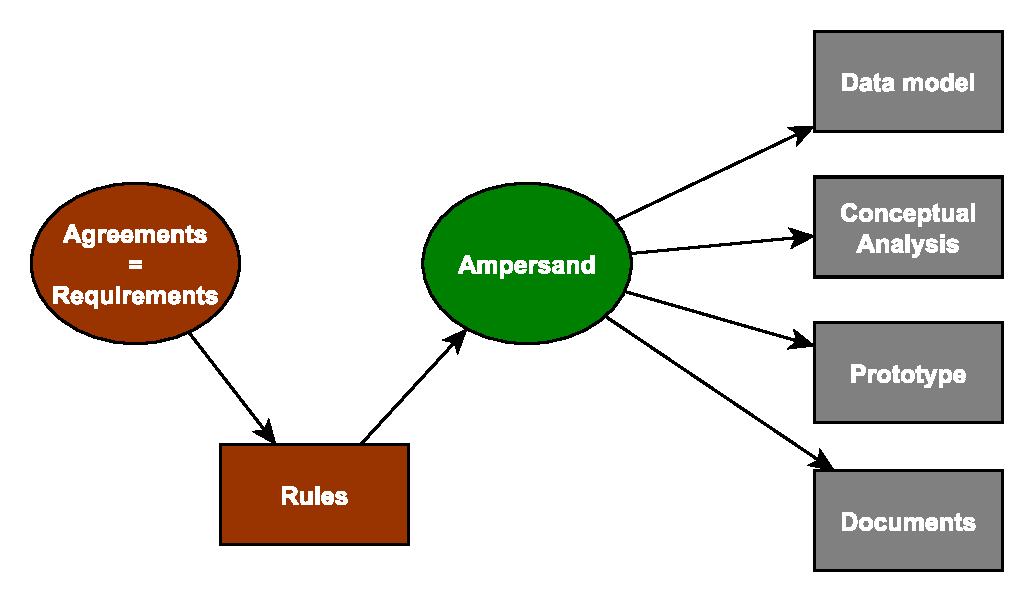
\includegraphics[width=0.7\textwidth]{Figures/Generation}
	\caption[Generated artifacts]{Ampersand generates several artifacts based on the business rules (source: \cite{ampersand-approach})}
	\label{fig:generation}
\end{figure}
%

The Ampersand project is used in several environments, by different user groups.
In a research context, the Ampersand project is part of the research on the use of business rules for software design.
In an educational context, it is also used as the main tool in the course `Rule Based Design' from the Open University of the Netherlands.
Finally, the compiler is used in business environments to design and develop real world business software.

% !TEX root = ../Thesis.tex

\subsection{High-level architecture}
\label{subsec:architecture}
The compiler developed for the Ampersand research project runs in several steps, hence the Ampersand compiler is also divided in several subcomponents:
\dict{P-structure}{The parse-tree generated by the Ampersand parser, used as input for the type checker}%
\dict{A-structure}{The ADL code generated by the Ampersand type checker, used as input for the calculator component}%
\dict{ADL-structure}{See A-structure}%
\dict{F-structure}{The functional structure generated by the Ampersand calculator, used as input for the different output modules}%
\begin{itemize}
	\item \textbf{Parser}: This component receives the ADL code as input, and parses that code into a parse-tree (also known as P-structure).
	\item \textbf{Type checker}: The Ampersand type checker receives a P-structure as input and converts it into a relational algebra format, suitable for manipulation (also known as A-structure or ADL-structure).
		 The semantics of ampersand are expressed in terms of the A-structure.
	\item \textbf{Calc}: The Calc component receives an A-structure as input, and manipulates it according to the research rules, generating the functional structure (also known as F-structure).
		The F-structure contains all design artifacts needed to write a specification and generate the output.
	\item \textbf{Output components}: All design artifacts present in the F-structure are ready to be rendered.
		Several components use this data structure to generate the wished output.
		The output components currently implemented (and their output formats) are the following: 
		\begin{itemize}
			\item Atlas (HTML interface);
			\item Revert (Haskell source);
			\item Query (prototype generation);
			\item Documentation Generator (Pandoc structure).
		\end{itemize}
\end{itemize}

% !TEX root = ../Documentation.tex

\subsection{Parser (R-M)}
\label{subsec:design-parser}
The mainstream design of the new parser has not changed much.
Basically, each EBNF rule receives its own parser function.
Thanks to the combinator operators, each parsing function also looks very similar to its corresponding EBNF.

The applicative interface is consistently used.
By changing details of the implementation, e.g. the order of the fields in the parse tree, we have made many of the `rebuild' functions unnecessary.
For some parsers the amount of changes necessary in order to remove supporting functions was too large or even impossible with the current parse tree.

Note that in parts of the parser, the function syntax has substituted the record syntax for creating data objects.
This was done only when the code readability could be improved by doing so.

\subsubsection{Parsec}
\label{subsec:design-parsing-lib}
As mentioned earlier, and described in research context document \citenac{parsing}, the new Ampersand parser has been rebuilt with another parsing library, namely Parsec.
However, for the Ampersand developers, the source code of the parser will still look very familiar, thanks to the applicative interface.
For developers, the main differences between Parsec and the uulib are:
\begin{itemize}
  \item Parsec does not backtrack by default.
    In order to enable backtracking, the \texttt{try} function must be used.
    This is described in \autoref{subsec:backtracking}.
  \item Parsec does not try to solve parsing errors.
    The parser stops immediately after the first issue.
    See also the error analysis in \autoref{subsec:design-errors}.
  \item Error messages are customizable by using the \texttt{<?>} operator.
    This is also suggested in \autoref{subsec:design-next-steps}.
  \item Some combinators have a different name, e.g. one must use \texttt{option} instead of \texttt{opt}.
    Assuming the documentation found on Hackage is clear and sufficient, interface differences are not documented here.
\end{itemize}

\subsubsection{Backtracking}
\label{subsec:backtracking}
In order to explain the differences on backtracking behavior between the uulib and Parsec, we quote here Doaitse Swierstra, the author of the uulib \citenac{swierstra-parsec}:
\begin{quote}
\textsl{To understand the subtleties it is important to understand the differences between the try construct in Haskell and the non-greedy parsing strategy used in uu-parsinglib. Effectively the latter is a try which just looks ahead one symbol. In that respect it is less powerful than the try construct from Parsec, in which you specify that a specific construct has to be present completely. And then there is the underlying different overall strategy. Parsec uses a back-tracking strategy with explicit tries to commit, whereas uu-parsinglib uses a breadth-first strategy with an occasional single symbol look-ahead.}
\end{quote}
%
We can therefore conclude that the try-statements in Parsec are undesirable.
However, they are necessary when the grammar is ambiguous.
In this section we explain why each of the remaining try statements are necessary, and how these issues can be resolved:
\begin{description}
  \item[Classify]
    This ambiguity in the grammar arises from the \texttt{Classify} and \texttt{GenDef} productions:
    \begin{quote}
        \texttt{Classify ::= `CLASSIFY' ConceptRef `IS' Cterm}\\
        \texttt{GenDef ::= (`CLASSIFY' | `SPEC') ConceptRef `ISA' ConceptRef}
    \end{quote}
    When the parser encounters \texttt{`CLASSIFY'}, it cannot define whether it found a \texttt{Classify} or a \texttt{GenDef} production.
    Therefore, the parser must consume the keyword and a \texttt{ConceptRef} before consuming either \texttt{`IS'} or \texttt{`ISA'} and determining which production is applicable.
    
    In order to solve this issue, one must choose a different keyword or symbol for each of the productions.
    Another option would be to merge the two statements in the same parser.
    We did not merge the productions because that would make the parser less maintainable.
  
  \item[Role]
    This ambiguity in the grammar arises from the \texttt{RoleRelation} and \texttt{RoleRule} productions:
    \begin{quote}
        \texttt{RoleRelation ::= `ROLE' RoleList `EDITS' NamedRelList}\\
        \texttt{RoleRule ::= `ROLE' RoleList `MAINTAINS' ADLidList}
    \end{quote}
    When the parser encounters \texttt{`ROLE'}, it cannot define whether it is a \texttt{RoleRelation} or a \texttt{RoleRule} production.
    Therefore, the parser must consume the keyword and a \texttt{RoleList} (which may be long) before consuming either \texttt{`MAINTAINS'} or \texttt{`EDITS'} and determining which production is applicable.
    
    In order to solve this issue, one must choose a different keyword for each of the productions, merge the two options to have the same representation in the parse tree, or refactor the parser so that the two options are parsed together.
    We did not merge the productions because that would make the parser less maintainable.
  
  \item[View]
    This ambiguity in the grammar arises from the \texttt{FancyViewDef} and \texttt{ViewDefLegacy} productions:
    \begin{quote}
        \texttt{FancyViewDef ::= `VIEW' Label ConceptOneRefPos `DEFAULT'? `\{' ViewObjList `\}' HtmlView? `ENDVIEW'}\\
        \texttt{ViewDefLegacy ::= (`VIEW' | `KEY') LabelProps ConceptOneRefPos `(' ViewSegmentList `)' }
    \end{quote}
    When the parser encounters \texttt{`VIEW'}, it cannot define whether it found a \texttt{FancyViewDef} or a \texttt{ViewDefLegacy} production.
    In this case, defining which construction is applicable is even more complicated.
    This decision must, in the worst case, be delayed until the parser encounters a \texttt{`\{'} or \texttt{'('}.
    That's because the productions \texttt{Label} and \texttt{LabelProps} are not disjoint, and \texttt{`DEFAULT'} is optional.
    
    In order to solve this issue, we advise to merge or drop the legacy statement.
    
  \item[Multiplicity]
    This ambiguity in the grammar arises from the \texttt{Mult} production:
    \begin{quote}
        \texttt{Mult ::= (`0' | `1') `..' (`1' | `*') | `*' | `1'}
    \end{quote}
    When the parser encounters \texttt{`1'}, it cannot define whether it found the first or the last production.
    The parser must therefore read the next token before choosing the right option.
    
    In order to solve this issue, we advise to refactor the grammar (and the parser) to have the following production:
    \begin{quote}
        \texttt{Mult ::= `0' `..' (`1' | `*') | `1'(`..' (`1' | `*'))? | `*'}
    \end{quote}
    %
    We did not refactor the code in this manner because the \texttt{pMult} parser does more than only parsing: it also changes the representation of the found constructions before creating the parse tree.
  
  \item[Labels and Terms]
    In the productions \texttt{Att} and \texttt{RuleDef}, we see very similar ambiguities:
    \begin{quote}
        \texttt{Att ::= LabelProps? Term}\\
        \texttt{RuleDef ::= `RULE' Label? Rule Meaning* Message* Violation?}
    \end{quote}
    Wherein:
    \begin{quote}
        \texttt{Label ::= ADLid ':'}\\
        \texttt{LabelProps ::= ADLid (`{' ADLidListList `}')? `:'}\\
        \texttt{Rule ::= Term ('=' Term | '|-' Term)?}
    \end{quote}
    And one of the possible productions of \texttt{Term} is:
    \begin{quote}
        \texttt{Term ::= Trm2 ::= Trm3 ::= Trm4 ::= Trm5 ::= Trm6 ::= RelationRef ::= NamedRel ::= Varid Sign?}
    \end{quote}
    While:
    \begin{quote}
        \texttt{ADLid ::= Varid | Conid | String}
    \end{quote}
    
    What happens here is that when the parser encounters a \texttt{Varid}, it cannot define whether it is part of the (optional) \texttt{Label} production or if no \texttt{Label} was given and the \texttt{Varid} is part of a \texttt{Term}/\texttt{NamedRel} production.
    
    Due to the quite complex grammar for the \texttt{Term} production, this issue may severely impact the parser's performance.
    This is probably the most harmful of the ambiguities mentioned.
    However, it can only be solved by adding a symbol before the \texttt{Term} production (e.g. making the `:' non-optional).
\end{description}
%
Please note that in order to have proper backtracking with correct error messages, Parsec may require two try-statements \citenac{try-harmful}.

% !TEX root = ../Thesis.tex

\subsection{Other objectives}
While designing and implementing the new Ampersand parser, the following objectives were also important:
\begin{itemize}
  \item \textbf{Integration}: The new parser must interface with the remaining Ampersand modules.
    It must thus be implemented in Haskell.
  \item \textbf{Libraries}: Since different implementation options are available, it was important to choose the most suitable Haskell parsing framework.
  \item \textbf{Maintainability}: Well-written and maintainable code is a must for the Ampersand project, since it is an open-source project.
    The maintainability must be either maintained or improved; otherwise the parser is not to be taken into production.
  \item \textbf{Tests}: Testing the parser well was a task for this project.
    The suggestion is to use testing tools to improve the process, e.g. QuickCheck.
  \item \textbf{Pretty-printing}: This is important in order to test the parser.
\dict{HPC}{Haskell Program Coverage}%
\dict{Haddock}{Software documentation generator for the Haskell programming language}%
\dict{HLint}{Statical analysis software that suggests maintainability improvements}%
  \item \textbf{Tools}: Within the Haskell community, several tools are popular to verify code quality and generate documentation, e.g. HPC, Haddock and HLint.
  \item \textbf{Fixed syntax}: The new parser must process the same inputs as the previous parser.
  \item \textbf{Fixed parse tree}: The new parser must produce the same outputs as the previous parser.
    Any further changes must be applied to the rest of the Ampersand system.
\end{itemize}

During the project, some additional requirements have been identified:
\begin{itemize}
  \item \textbf{Git/GitHub}: The changed software had to be integrated into the GitHub Ampersand project.
    The development itself happened in a separate branch of a separate fork, so that deliveries could be merged in a smooth way.
    This was an especially hard requirement for us, since we had no experience with Git.
  \item \textbf{Cabal}: The building system for Haskell had to be maintained as the building platform.
  \item \textbf{EBNF}: The syntax of the Ampersand grammar was specified in EBNF notation but was not up-to-date.
    Any changes to the syntax had to be documented according with this notation.
    One option was to add the EBNF as comment in the source code in order to make clear that the complete grammar is implemented correctly.
\end{itemize}

On top of the project goals, we also wanted to help the university and other students with our results.
Finally, building up knowledge was also important for us (i.e. functional programming, Haskell, compilers, parsers, LaTeX, Ampersand, business rules and research in general).


% !TEX root = ../Thesis.tex

\section{Domain \& techniques}
\label{sec:domain}
% !TEX root = ../Thesis.tex

%algemeen overzicht domeinen en technieken plusminus 2 pagina's
\subsection{Overview}
\lipsum[3]

% !TEX root = ../Thesis.tex

% individueel verslag onderzoek deeldomein en bijhorende technieken, plusminus 5 pagina's
% details van domein en technieken in relatie met het onderzoeksproject
% academische verantwoording gemaakte keuzen

\subsection{The Ampersand Approach (M)}
\label{domain:approach}
\lipsum[1]

\documentclass[a4paper,12pt,abstracton,titlepage]{scrartcl}
\usepackage{scrpage2}
\usepackage[utf8]{inputenc}
\usepackage[T1]{fontenc}
\usepackage[top=2.5cm, bottom=2.5cm, left=2cm, right=2cm]{geometry}
\usepackage[affil-it]{authblk}
\usepackage{lipsum}
\usepackage{url}
\usepackage[hidelinks]{hyperref}
\usepackage{graphicx}
\usepackage[table,xcdraw]{xcolor}
\usepackage{longtable}
\usepackage{multicol}

%citations
\usepackage{multibib}
\newcites{ac}{Academic references}
\newcites{nac}{Informal references}

% code for generating glossary, from http://tex.stackexchange.com/a/5837/59718
\usepackage[acronym,toc]{glossaries}
\usepackage{glossary-mcols}
\newcommand{\dict}[2]{%
  \newglossaryentry{#1}{name=#1,description={#2}}%
  \glslink{#1}{}%
}
\makeglossaries

% Here we set up the header, meta-information and front matter
%\date{December 17, 2014}      %// Today's date will appear when this is commented out.
\newcommand{\version}{0.3}

% title page
\author{Daniel S. C. Schiavini}
\affil{Open Universiteit Nederland, faculteit Informatica \\
	T61327 - Afstudeerproject bachelor informatica}
\title{Haskell parsing libraries \&\\ user-friendly error messages}
\subtitle{Useful feedback in the Ampersand parser\\
	~\\
	Phase 3a: Domain \& Techniques}
\publishers{Version \version}

% header
\pagestyle{scrheadings}
\setheadsepline{0.2pt}
\clearscrheadings
\automark[section]{chapter}
\ihead{Daniel S.C. Schiavini}
\ohead{Parsing libraries \& error messages}
\cfoot{\pagemark}

% URL's
\renewcommand*{\UrlFont}{\footnotesize\ttfamily}

% hyphenation
\hyphenation{
	gua-ran-tee
	pro-duct
	cor-res-pon-ding
	me-cha-nism
	know-ledge
	de-ve-lo-pers
	do-cu-men-ta-tion
	sa-tis-fac-tion
	Schi-a-vi-ni
	Ba-ert-so-en}

% Now the document starts
\begin{document}
\maketitle
\newpage

\tableofcontents
%\listoffigures
%\listoftables
\clearpage

% !TEX root = ../Documentation.tex
\section{Introduction}
\subsection{Identification}
This document contains the domain \& techniques analysis of the project `Useful feedback in the Ampersand parser'.
The document is the milestone product of the project phase 3a for Daniel S.C. Schiavini, as specified in the project planning \citenac{plan}.

This document is part of the graduation project of the computer science bachelor at the Open Universiteit Nederland.
The project `Useful feedback in the Ampersand parser' is executed in collaboration with Maarten Baertsoen, with support of the supervisor Dr. Bastiaan Heeren and examiner Prof.dr. Marko C.J.D. van Eekelen.
The assignment is given by Prof.dr. Stef Joosten, who researches how to further automate the design of business processes and information systems by the development of the Ampersand project.

Ampersand is an approach for the use of business rules to define the business processes.
Users describe the business rules in a formal language (ADL), and Ampersand compiles those rules into functional specification, documentation and working software
prototypes.
The main objective of this project is to improve the feedback and maintainability of the Ampersand parser.
See \citenac{plan} for more details on the project.

\subsection{Goals}
\lipsum[3]

\subsection{Document overview}
\lipsum[4]
% !TEX root = ../Parsing.tex

\section{Haskell parsing libraries}
\label{sec:libraries}

\subsection{Parsing remarks}
\dict{Lexical analysis}{Separating text into tokens}%
\dict{Lexer}{Software that does the lexical analysis}%
\dict{Alex}{Lexer included in the Haskell Platform}%
Parsing is sometimes divided into two stages: lexical analysis (separating the source text into tokens) and parsing itself (constructing a parse tree).
Tools such as the ones analyzed here can perform both lexical analysis and parsing.
However, sometimes the tools can be more efficient when supported by a separate Lexer (e.g. Alex).

Grammars associated with a formal language are described as a set of production rules.
Since these rules are formally defined, a series of mathematical constructions can be used to manipulate and describe the grammar.

\dict{ADL}{Ampersand Definition Language}%
\dict{BNF}{Backus-Naur Form, a meta-syntax notation for expressing context-free grammars}%
\dict{EBNF}{Extended Backus-Naur Form, an extension on BNF}%
The Ampersand Definition Language (ADL) is specified in a grammar in the Extended Backus-Naur Form (EBNF).
Even though it is known that the grammar is not up to date, this article assumes the updated version will not fundamentally be different than the specified grammar.

\subsection{Generators vs. combinators}
\dict{DSL}{Domain specific language}%
Generally, there are two options for implementing a parser:
The first option is to implement the parser in the language of choice, i.e. Haskell for this project.
Another possibility is to use a domain-specific-language (DSL) to describe the grammar, and let a separate software generate the actual parsing code.
The two approaches and their advantages and disadvantages are described in this section.

\subsubsection{Parsing libraries}
When programmers go down the path of building a parser directly in Haskell, building up a set of functions that support parsing is a natural consequence.
Although it's possible to build these functions for each and every project \cite{monadic-parsing}, using a premade library has several advantages, e.g. reduced effort, increased functionality, optimized performance and better documentation.
The extra effort to learn the library is paid off by these advantages.
In Haskell this is mostly done by providing monadic combinators to hold up extra information about the parsing state, and results in very elegant solutions \cite{monadic-parsing}.

The parsers built in Haskell are mostly recursive descent parsers, wherein the parser runs top-down from a set of recursive calls.
The program structure is then closely related to the production rules, supporting the readability of the program structure.

These parsers analyze the input text from \underline{L}eft to right and choose the \underline{L}eftmost derivation in the grammar.
Such parsers are called therefore LL parsers.

~\\
However, there are limitations related to recursive descent parsers.
For instance, a common kind of production rule is a left recursive one, e.g. \texttt{term $\rightarrow$ term `$+$' term $|$ digit}.
In this case, the first thing the parser would do is call itself, resulting in an infinite loop.
Gladly, left recursive grammars can be converted into right recursive ones \cite{remove-left}.

Therefore, LL parsers may require exponential time to run and are not able to guarantee termination.
In order to guarantee termination and linear execution time, a recursive descent parser must be able to recognize which production rule to use by reading only limited amount of tokens.
This is only possible for the class of unambiguous grammars without left recursion.

~\\
\dict{LL(k)-grammar}{A grammar that can be parsed by an LL($k$)-parser}%
\dict{LL(k)-parser}{Top-down parser that parses from left to right, performing the leftmost derivation with a maximum $k$-tokens of look-ahead}%
The EBNF for the ADL-language is not ambiguous and has no left recursion.
This grammar can therefore be called an LL($k$)-grammar, for which an LL($k$)-parser can be created.
The $k$ between the parenthesis means that this parser needs a maximum of $k$ tokens of look-ahead in order to choose a production rule.

\subsubsection{Parser generators}
As mentioned, another approach for building a parser is to specify the software's grammar in a specific notation and use a parser generator to create the actual parser source code.
In the domain of context-free grammars, a widely used grammar notation is the Backus-Naur Form (BNF).

\dict{Happy Parser Generator}{Parser generator system for Haskell. \url{https://www.haskell.org/happy/}}%
This research is focused in the Happy parser generator, which is part of the Haskell Platform since 2001.
Happy inputs a file containing an annotated BNF specification of a grammar and produces a Haskell module with a parser for that grammar.
Since it is possible to convert EBNF to BNF \cite{convert-ebnf,bnf-ebnf}, a Happy parser should not involve a lot of effort.
It is important to know, however, that besides converting the EBNF to BNF, the annotation still requires effort and knowledge acquisition.

\dict{LR parser}{Top-down parser that parses from left to right, performing the rightmost derivation}%
A parser generator is able to execute statical analysis on the input grammar.
Besides, they are often able to recognize more complicated grammars by running \underline{L}eft-to-right, and picking the \underline{R}ightmost derivation, being called therefore an LR parser.

\dict{LALR parser}{LR parser with look-ahead}%
An LR parser with \underline{L}ook-\underline{A}head is called an LALR parser.
By performing the rightmost derivation of the production rules, an LALR parser is able to recognize more complex grammars.
However, its workings are quite unintuitive, and understanding such parsers can be very hard.
That's exactly why LALR parsers are usually generated instead of built by hand.

Since understanding LALR parsers is hard, the syntax errors caused by incorrect input may be much harder to pinpoint and understand.
The errors generated by LALR parsers are often not in high-level terms that the end users can understand.

\dict{GHC}{Glasgow Haskell Compiler}%
\dict{Hugs}{Haskell Compiler}%
\dict{YACC}{Yet Another Compiler Compiler}%
\dict{Hellium}{Haskell Compiler}%
\dict{GCC}{Gnu Compiler Collection}%
Haskell compilers GHC and Hugs are both built with LALR generated parsers: Hugs is written in YACC and GHC is built with Happy \cite{hugs-parser,ghc-parser}.
Later on, the Helium compiler was created for classroom-use because the mentioned Haskell compilers were not user friendly \cite{helium-parser}.
Other examples are the GCC compilers for C and C++, that started as LALR generated compilers and were remade to be recursive-descent parsers \cite{gcc-c-parser,gcc-cpp-parser}.

Although it's harder to understand its workings, the resulting source code for the generators is simpler and easier to maintain, as can be seen in \cite{parser-examples}.

\subsubsection{Conclusion}
In the context of the new Ampersand parser, some advantages of building the parser in Haskell instead of using a generator, are:
\begin{description}
	\item[Flexibility] The programming language gives much more flexibility in coping with context-sensitive grammars.
	\item[Building] The process is simpler since it is unnecessary to run a separate program to generate the parser.
	\item[Language] Both the customer and the project members feel more comfortable working in Haskell then in an unknown DSL.
	\item[Errors] The main objective of the project is giving useful feedback in the new Ampersand parser, and this seems much easier to achieve with a handwritten parser.
\end{description}

\noindent
On the other hand, the advantages of using a parser generator, instead of handwriting the code, are:
\begin{description}
	\item[Optimizations] Because the parser is generated on-the-fly, the generator can apply optimizations that would otherwise be hard to implement.
	\item[Performance] Bottom-up parsers are much more efficient because they are able to pack the code into state machines.
		This is even more valid when many parsing alternatives are available.
	\item[Static analysis] The generator is able to do a lot more static analysis, while a library is only executed during the run-time.
    E.g. programmers will only know of left recursions and non-terminations by testing the parser.
	\item[Documentation] Since the DSL is basically annotated BNF, keeping the syntax diagrams up to date is much easier.
\end{description}

\noindent
From the above advantages and disadvantages, it is clear that no universal truth exists in these matters.
Although it is a difficult choice, the error messages are indeed the most important project target, so writing the parser by hand is the advised option.
This choice also means that it keeps on being a task of the developers to update the documentation, e.g. the syntax diagrams that are currently not up-to-date.

\subsection{Combinator libraries}
In the previous section, the choice to use a combinator library has been taken.
In this section, two libraries will be compared: the Utrecht University parser combinator library (uu-parsinglib) and Parsec.
Other libraries (e.g. Attoparsec, Polyparse) are out of the scope of this research.

\subsection{Utrecht University Parsing Library}
\dict{uu-parsinglib}{Haskell parsing library from the Utrecht University. \url{http://foswiki.cs.uu.nl/foswiki/HUT/ParserCombinators}}%
The uu-parsinglib is a combinator library created by Doaitse Swierstra in the Utrecht University.
This library is used in many mature projects.
The current Ampersand parser is also built with the previous version of the uu-parsinglib.
The new version has several improvements, mainly in performance \cite{benchmark}.
It currently has more than 4 thousand downloads in the Hackage package manager.

The documentation is mainly in Haddock format and in a paper from 2009 \cite{uu-doc}.
The implementation is open source.
The new version of the uu-parsinglib provides combinators that include error correction and a monadic interface.
Errors are recognized and corrected automatically if the programmers want so, but the reporting is customizable.
It also supports grammars that are not context-free and even ambiguous grammars (provided the user accepts exponential run-time).

Finally, the uu-parsinglib runs online, i.e. it returns parts of the parsing three as soon as they are ready.
This gives programmers the ability to do lazy parsing.

\subsection{Parsec}
\dict{Parsec}{Haskell monadic parsing combinator library written by Daan Leijen. \url{https://www.haskell.org/haskellwiki/Parsec}}%
Parsec is a monadic parsing combinator library created by Daan Leijen, while also working at the Utrecht University.
It seems to be the most popular combinator library in the Haskell community, with more than 200 thousand downloads in the Hackage package manager.

Parsec is designed to be simple, safe and well documented industrial parser library.
Besides, there has also been some work done on the performance and error messages.
The documentation of Parsec and its documentation tends to be better than that of the uu-parsinglib because of a larger user base.

%todo: this section is very empty
%todo: https://www.haskell.org/haskellwiki/Parsec
%todo: http://stackoverflow.com/questions/19208231/attoparsec-or-parsec-in-haskell/19213247#19213247

\subsection{Monadic vs. arrow interfaces}
Monads allow sequences and state to be saved during the parsing, and had become the most common way of building Haskell parsers.
Until, in a paper from Swierstra \cite{error-correcting}, a parsing library was published with an alternative interface.
Hughes presented this alternative as a generalization of monads, calling it `arrows' \cite{monad-arrows}.

Arrows are less convenient than monads but are much widely applicable \cite{monad-arrows}.
Monads would still be used for state passing and other constructions, but the continuations would be carried over to arrows.

Arrow-style parsers do not depend on the run-time values -- they are not dependent on the context.
This means that it is then possible to analyze and optimize the parser before executing it.
Swierstra goes so far to say that this works as a run-time parser generator \cite{error-correcting}.
On the other hand, the lack of context means that only context-free languages can be implemented this way \cite{parsec}.

The uu-parsinglib allows both monadic and arrow-style parsing, while Parsec only has a monadic interface.
In the arrow-style interface, the uu-parsinglib also adds error correction:
After detecting an error, the library will correct it by adding or deleting tokens.
It then generates an appropriate error message and continues with the rest of the program.
By using this interface, the parsing will thus always succeed.

%todo: http://worldbusiness.org/wp-content/uploads/2012/10/arrows-and-idioms2.pdf
%todo: http://marc.info/?l=haskell-cafe&m=128039136131494

\subsection{Conclusion}
The following differences have been found between the two considered libraries:
\begin{description}
	\item[Documentation] The documentation of Parsec seems to be more extended and well-maintained.
		Several Parsec tutorials can be found on the internet (e.g. \cite{using-parsec}).
		On the other hand, the uu-parsinglib's documentation is mostly generated from code annotations.
	\item[Support] Since Parsec is much more used, online support can be more easily found.
		For example, the website Stack Overflow currently has 14 questions about the uu-parsinglib and 301 about Parsec.
	\item[Static checking] None of the libraries is able to do static checking.
		However, the uu-parsinglib has more possibilities of grammar analysis in its arrow-style interface.
	\item[Precedences] The Ampersand parser is currently built with the uu-parsinglib with great satisfaction.
		This both means that the library has enough features and that it is known by the other Ampersand developers.
	\item[Error reporting] No literature has been found with a comparison of the errors generated by the libraries.
		However, many publications affirm that the generated errors from both libraries are great \cite{helium-parser,benchmark,uu-doc,error-correcting,parsec}.
	\item[Error recovery] When a parsing error is found, a Parsec parser stops immediately.
		A parser built with uu-parsinglib, however, corrects the error and continues parsing.
		Error correction is good because the parser always succeeds.
		On the other hand, a big list of errors can also overwhelm the user \cite{heeren-error}.
		Finally, to perform the corrections, the parser needs to make assumptions based e.g. on statistics;
		these assumptions cannot always be correct.
	\item[Fine-tuning] According to the Helium development team, Parsec's possibilities for error fine-tuning are greater \cite{helium-parser}.
		However, to apply optimizations it is necessary to know the internal workings of the parser \cite{uu-doc}.
	\item[Backtracking] Parsec works with more traditional backtracking algorithms \cite{parsec} that can often lead to high space consumption \cite{uu-doc}.
		Backtracking must be manually activated, though.
	\item[Performance] The Parsec library seems to have better performance \cite{benchmark}, but the difference is small and is not expected to make a considerable difference in the small ADL scripts.
	\item[Try operator] In order to allow backtracking, Parsec code uses the try-function, which is considered harmful and can be easily misused \cite{try-harmful}.
		This keyword is totally unnecessary in the uu-parsinglib because it uses breadth-first lazy parsing \cite{uu-doc}.
		%todo: http://osdir.com/ml/haskell-cafe@haskell.org/2012-01/msg00566.html
	\item[Maintainability] No significant difference has been found in the maintainability of the two analyzed libraries.
		Note that the programmers working on Ampersand are already familiar with the uu-parsinglib.
		On the other hand, there is more support and documentation available for Parsec, so it can also be seen as more future-proof.
		The responsibility for the maintainability still lies on the hands of the programmers building the parser.
	\item[Origin] Both libraries are originated at the Utrecht University.
		In 2003, a Haskell compiler focused on user friendliness, Helium, was published from the same university.
		Knowing both libraries very well, the authors made the choice to use Parsec because of the possibilities of error customization \cite{helium-parser}.
\end{description}
%
Considering these differences, a deeper analysis of error messages is given in the next section.
The actual library choice is delayed until \autoref{sec:conclusion}.

% !TEX root = ../Thesis.tex

\subsection{Errors}
\label{analysis:errors}
%TODO: Bastiaan suggests we should try to use the definition of the error manifesto by Yang et al. (page 32 of his doctor)
In this section, we analyze the error messages given by the previous parser.
The results of this analysis are compared with the new parser in \autoref{tests:errors}.

\subsubsection{Error message qualification}
The user friendliness and correctness of an error message is a subjective topic and therefore we need to start with a definition to objectively judge the quality of an error message.
After analyzing the current Ampersand parser error messages, we identified the following objective aspects of an Ampersand parser error message:
%
\begin{description}
	\item [Position]
	Each error messages reports the correct position (file, line number and column) of where the user committed the error.
	\item [Accuracy]
	The accuracy of an error message is measured based upon the following characteristics:
	\begin{enumerate}
		\item	\textbf{\small How does the provided error description outline the discovered error:}
				Providing the user with a good description of the encountered syntax issue will support a fast error resolution.
				When the issue is vaguely described without pinpointing the exact issue, the error resolution will be time consuming.
		\item	\textbf{\small Pinpointing the correct error}:
				An error can lead to multiple subsequent issues.
				These issues are, however, irrelevant for the user and the Ampersand parser should provide the exact origin of the issues.
		\item	\textbf{\small Quality of the hint:}
			The message can provide a hint for a solution together with the error message to support the user with the error resolution.
	\end {enumerate}
    \item[Conciseness]
	Providing a good error description is one thing, but this one message can be hidden between several other error messages that result from the initial error.
	It is unlikely that users will easily find the exact originating issue in their source file when they are overwhelmed with a multitude of error messages. % using plural to avoid repeating his/her
\end {description}
%
Based on these objective properties to judge the quality of the parsing errors, we defined the following criteria to distinguish between good, bad and average (but acceptable) error messages:
%
%TODO: Bastiaan doesn't think there's a main originating error. See his review in page 15.
\begin{description}
	\item [Bad error message] A message is considered to be bad if one of the criteria below is fulfilled:
		\begin{description}
			\item [Position]
			The position has a deviation of more than one line or ten column positions from where the actual error is made.
			\item [Accuracy]~
				\begin{itemize}
					\item 	The provided error description is useless for the user to determine the actual error.
					\item 	The provided error description is not appointing the main, originating error without any correlation towards this main error.
				\end {itemize}
			\item[Conciseness]
			More than distinct three errors are mentioned by the Ampersand parser.
		\end {description}
	\item [Acceptable error message] A message is considered to be of average, but acceptable, quality if one of the criteria below is fulfilled:
		\begin{description}
			\item [Position]
			The position has a deviation between five and ten column positions from where the actual error is made.
			\item [Accuracy]~
				\begin{itemize}
					\item 	The provided error description is not an exact description of the error, but provides 6useful information to discover the actual issue.
					\item 	The provided error description is not appointing the main originating error, but the link to the actual error can be discovered based on the provided information.
					\item 	The provided hint is incorrect.
				\end {itemize}
			\item[Conciseness]
			two or three errors are mentioned by the Ampersand parser.
		\end {description}
		
	\item [Good error message] Any error message that is not bad nor acceptable is good.
\end {description}

\subsubsection{Gathering process}

To gather the necessary input for the as-is analysis, an exhaustive list of all possible error messages is created.
This as-is analysis will be used as a reference base to verify the implementation of the new error mechanism with Parsec.
The errors are invoked by simulating all possible syntax errors that will invoke an error within the Ampersand parser.
Each syntax statement is therefore manipulated, introducing one specific error per time, and the resulting error message is then recorded together with the actual erroneous statement.
The exact same statements are afterwards pushed through the new parser, making it possible to make a quantitative `before and after' analysis.
Special attention is given to avoid redundant errors that could influence the quantitative analysis. 
An example of such an redundant error is the use of a capital letter in defining a specific reference. 
Although these references are used in several syntax statements, there is only one procedure in the parser to check all references starting with a capital letter.
An improvement in the error message of this check may only be taken into account one time.

\subsubsection{Results}
Based on our error message qualification definition, \autoref{tab:error-messages-analysis} visualizes the results of the as-is analysis.
This analysis clearly confirms the statement that the quality of the error messages is of low quality and that there is a lot of room for improvement.

% Please add the following required packages to your document preamble:
% \usepackage[table,xcdraw]{xcolor}
% If you use beamer only pass "xcolor=table" option, i.e. \documentclass[xcolor=table]{beamer}
\begin{table}[h]
  \centering
	\begin{tabular}{llrlr}
    Error quality  & \multicolumn{2}{c}{Previous parser}     \\
		Good           & 19          & 22,35\%         \\
		Acceptable        & 48          & 56,47\%       \\
		Bad            & 18          & 21,18\%           \\
		\rowcolor[HTML]{BBBBBB}
		\textbf{Total} & \textbf{85} & \textbf{100,00\%} 
	\end{tabular}
  \caption{Error message as-is analysis results}
  \label{tab:error-messages-analysis}
\end{table}

% !TEX root = ../Parsing.tex

\section{Conclusion}
\label{sec:conclusion}
In \autoref{sec:libraries}, the advice was given to use a combinator library for the new parser of Ampersand.
The main reason to avoid the parser generators is that it is hard to generate useful feedback.
Then, in \autoref{sec:errors}, it was made even more clear that besides generating good messages, those messages should also be customizable.

Therefore, the advice of this research is to use the combinator library that offers the highest level of customization in error messages, Parsec.
Although the uu-parsinglib seems to also be a very good choice, the experiences from the Helium compiler \citeac{helium-parser} should be also considered.
Besides, the Parsec library offers better support.

A list of important consideration points has also been collected through the literature and can be found in \autoref{sec:errors}, more specifically \ref{subsec:errors-ampersand}.

\part*{Appendices}
\addcontentsline{toc}{part}{Appendices}
\appendix
% !TEX root = ../Parsing.tex

\small
\printglossary[style=mcolindex,title=Glossary]
\label{sec:glossary}

% !TEX root = ../Parsing.tex
\addcontentsline{toc}{section}{References}
\label{sec:bibliography}

\begin{thebibliography}{99}

\bibitem{plan}
	Planning for the project `Useful feedback in the Ampersand parser'\\
	Maarten Baertsoen and Daniel S. C. Schiavini\\
	Version 2.0 -- November 29, 2014\\
	\url{http://git.io/NeHuLg}

\bibitem{heeren-error}
	Top Quality Type Error Messages\\
	Bastiaan Heeren\\
	ISBN 90-393-4005-6, September 20, 2005\\
	\url{http://www.open.ou.nl/bhr/phdthesis}

\bibitem{monadic-parsing}
	Functional pearls -- Monadic Parsing in Haskell\\
	Graham Hutton (University of Nottingham) and Erik Meijer (University of Utrecht)\\
	\url{http://www.cs.nott.ac.uk/~gmh/monparsing.pdf}

\bibitem{convert-ebnf}
	 From EBNF to BNF \\
	 Christoph Zenger\\
	 June 4, 2000\\
	 \url{http://lampwww.epfl.ch/teaching/archive/compilation-ssc/2000/part4/parsing/node3.html}

\bibitem{bnf-ebnf}
	BNF and EBNF: What are they and how do they work?\\
	Lars Marius Garshol\\
	August 22, 2008\\
	\url{http://www.garshol.priv.no/download/text/bnf.html}

\bibitem{parser-examples}
	Haskell Parser Examples\\
	Geoff Hulette\\
	August 22, 2014\\
	\url{https://github.com/ghulette/haskell-parser-examples}

\bibitem{hugs-parser}
	Source code of the Hugs parser\\
	March 25, 2007\\
	\url{https://github.com/fuzxxl/Hugs/blob/master/src/parser.y}

\bibitem{ghc-parser}
	GHC: The Parser\\
	December 1, 2014\\
	\url{https://ghc.haskell.org/trac/ghc/wiki/Commentary/Compiler/Parser}
	%\url{https://ghc.haskell.org/trac/ghc/browser/ghc/compiler/parser/Parser.y}
	%https://www.haskell.org/pipermail/haskell-cafe/2013-August/109557.html

\bibitem{helium-parser}
	Helium, for Learning Haskell\\
	Bastiaan Heeren, Daan Leijen, Arjan van IJzendoorn\\
	Utrecht University\\
	\url{http://www.open.ou.nl/bhr/heeren-helium.pdf}
	
\bibitem{gcc-c-parser}
	GCC 4.1 Release Series Changes, New Features, and Fixes\\
	\url{https://gcc.gnu.org/gcc-3.4/changes.html}

\bibitem{gcc-cpp-parser}
	GCC 3.4 Release Series Changes, New Features, and Fixes\\
	\url{https://gcc.gnu.org/gcc-4.1/changes.html}
	
\end{thebibliography}

\end{document}
% !TEX root = ../Thesis.tex

\subsection{Context (M)}
\dict{Test}{Testing glossary}%
\begin{description}
	\item [Customer] Stef Joosten
	\item [Supervisor] Bastiaan Heeren
	\item [Research context] Modelleren van bedrijfsregels
	\item [Programming language] Haskell
\end{description}

\begin{itemize}
	\item Refactoren van de source code van een parser uit een open source project 
	\item Verbeteren van de parser-foutmeldingen
\end{itemize}

% !TEX root = ../Thesis.tex

%beschrijving van het opgeleverde eindproduct, plusminus 15 pagina’s

\section{Results}
beschrijving van het projectresultaat (het softwaresysteem)
overzicht van de oplossing, met enkele globale voorbeelden

% !TEX root = ../Thesis.tex

\section{Assessment}
reflectie inhoud, resultaat
beperkingen in het resultaat/afbakening (op voorhand en praktisch) 


% !TEX root = ../Parsing.tex

\section{Conclusion}
\label{sec:conclusion}
In \autoref{sec:libraries}, the advice was given to use a combinator library for the new parser of Ampersand.
The main reason to avoid the parser generators is that it is hard to generate useful feedback.
Then, in \autoref{sec:errors}, it was made even more clear that besides generating good messages, those messages should also be customizable.

Therefore, the advice of this research is to use the combinator library that offers the highest level of customization in error messages, Parsec.
Although the uu-parsinglib seems to also be a very good choice, the experiences from the Helium compiler \citeac{helium-parser} should be also considered.
Besides, the Parsec library offers better support.

A list of important consideration points has also been collected through the literature and can be found in \autoref{sec:errors}, more specifically \ref{subsec:errors-ampersand}.
\newpage

% !TEX root = ../Thesis.tex

\appendix
\addcontentsline{toc}{part}{Appendices}
% !TEX root = ../Parsing.tex

\small
\printglossary[style=mcolindex,title=Glossary]
\label{sec:glossary}

\clearpage
% !TEX root = ../Parsing.tex
\addcontentsline{toc}{section}{References}
\label{sec:bibliography}

\begin{thebibliography}{99}

\bibitem{plan}
	Planning for the project `Useful feedback in the Ampersand parser'\\
	Maarten Baertsoen and Daniel S. C. Schiavini\\
	Version 2.0 -- November 29, 2014\\
	\url{http://git.io/NeHuLg}

\bibitem{heeren-error}
	Top Quality Type Error Messages\\
	Bastiaan Heeren\\
	ISBN 90-393-4005-6, September 20, 2005\\
	\url{http://www.open.ou.nl/bhr/phdthesis}

\bibitem{monadic-parsing}
	Functional pearls -- Monadic Parsing in Haskell\\
	Graham Hutton (University of Nottingham) and Erik Meijer (University of Utrecht)\\
	\url{http://www.cs.nott.ac.uk/~gmh/monparsing.pdf}

\bibitem{convert-ebnf}
	 From EBNF to BNF \\
	 Christoph Zenger\\
	 June 4, 2000\\
	 \url{http://lampwww.epfl.ch/teaching/archive/compilation-ssc/2000/part4/parsing/node3.html}

\bibitem{bnf-ebnf}
	BNF and EBNF: What are they and how do they work?\\
	Lars Marius Garshol\\
	August 22, 2008\\
	\url{http://www.garshol.priv.no/download/text/bnf.html}

\bibitem{parser-examples}
	Haskell Parser Examples\\
	Geoff Hulette\\
	August 22, 2014\\
	\url{https://github.com/ghulette/haskell-parser-examples}

\bibitem{hugs-parser}
	Source code of the Hugs parser\\
	March 25, 2007\\
	\url{https://github.com/fuzxxl/Hugs/blob/master/src/parser.y}

\bibitem{ghc-parser}
	GHC: The Parser\\
	December 1, 2014\\
	\url{https://ghc.haskell.org/trac/ghc/wiki/Commentary/Compiler/Parser}
	%\url{https://ghc.haskell.org/trac/ghc/browser/ghc/compiler/parser/Parser.y}
	%https://www.haskell.org/pipermail/haskell-cafe/2013-August/109557.html

\bibitem{helium-parser}
	Helium, for Learning Haskell\\
	Bastiaan Heeren, Daan Leijen, Arjan van IJzendoorn\\
	Utrecht University\\
	\url{http://www.open.ou.nl/bhr/heeren-helium.pdf}
	
\bibitem{gcc-c-parser}
	GCC 4.1 Release Series Changes, New Features, and Fixes\\
	\url{https://gcc.gnu.org/gcc-3.4/changes.html}

\bibitem{gcc-cpp-parser}
	GCC 3.4 Release Series Changes, New Features, and Fixes\\
	\url{https://gcc.gnu.org/gcc-4.1/changes.html}
	
\end{thebibliography}

\end{document}